\documentclass[whitelogo, table, oneside]{template/tudelft-report}
\usepackage[utf8]{inputenc}
\usepackage{changes}
\usepackage{graphicx}
\usepackage{adjustbox}
\usepackage{listings}
\usepackage{ragged2e}
\usepackage{pgfgantt}
\usepackage[normalem]{ulem}
\usepackage{pdflscape}
\usepackage{wrapfig}
\usepackage{comment}
\usepackage{enumitem}
\definecolor{hague-limegreen}{RGB}{158, 167, 0}
\definecolor{hague-grey}{RGB}{51, 63, 72}
\usepackage[parfill]{parskip}

\begin{document}
\frontmatter
\begin{titlepage}

 \newgeometry{left =0cm, right =0cm,bottom = 0cm, top = 0.5 cm  }
 \pagecolor{hague-limegreen}
    
    
    \newcommand{\kantlinebreedte}{1cm}
    % \newcommand{\dedatum}{11 September 2021}
    \newcommand{\dedatum}{\today}
    \newcommand{\detitel}{Plan of Approach}
    \newcommand{\desubtitel}{LIDAR Camera Synchronisation}
    
    \begin{flushleft}
        \huge 
        \hspace{0,9 cm} \\ 
        \hspace{0,9cm} {\fontsize{50}{60}\selectfont\detitel\\}
        \hspace{\kantlinebreedte}
        \textcolor{black}{\desubtitel\\}
        
        \vspace{1cm}
        
        \begin{figure}[h]
        \centering
        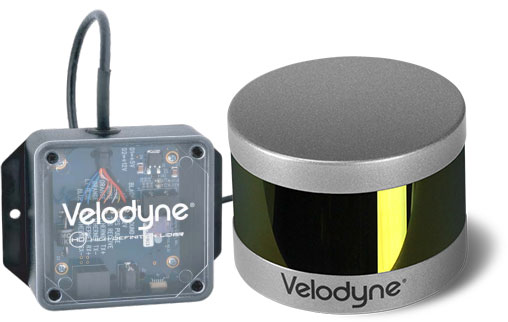
\includegraphics[width=\textwidth]{cover/image_lidar.png}
       
        \end{figure}
        
        \vspace{0.6cm}
        
        \Large
        \hspace{\kantlinebreedte}
        \textcolor{black}{Van Driel, Bas (17137640)\\}
        \hspace{\kantlinebreedte}
        \textcolor{black}{Swinkels, Bob (18057519)\\}
        \hspace{\kantlinebreedte}
        \textcolor{black}{Van Straaten, Luca (18073611)\\}
        \hspace{\kantlinebreedte}
        \textcolor{black}{Louwes, Bart (17018994)\\}
        \hspace{\kantlinebreedte}
        \textcolor{black}{Electrical Engineering\\}
        \hspace{\kantlinebreedte}
        \textcolor{black}{supervisor: S.D. O’Loughlin\\}
        \hspace{\kantlinebreedte}
        \textcolor{black}{client: F. Garcia Fernandez\\}
        \hspace{\kantlinebreedte}
        \textcolor{black}{\dedatum \\}
        \hspace{\kantlinebreedte}
        \textcolor{black}{Version: 1}
        
        
        \end{flushleft}
        
        \begin{figure}[h]
        \centering
        
\includegraphics[right, scale=0.83]{cover/logo_black.pdf}
        \end{figure}




\end{titlepage}

\pagecolor{white}

\tableofcontents

\mainmatter

\chapter{Background}

The Smart Sensors Systems (S3) research-group is developing a sensor suite capable of detection and classification for robotics applications in collaboration with industry and academic partners. Sensors such as LiDAR and cameras are required for these robotics applications.

\section{Problem definition}

Smart Sensors Systems is working on a sensor suite, using LIDAR and camera's to
detect and classify objects. For various reasons, it is important that the
frames of the LIDAR and camera are captured at the same time. We are tasked
with designing electronics that can capture the frames at the same time. And
timestamp them accordingly.
 % luca
\chapter{Project Results}
\label{ch:results}
This chapter seeks to provide a concrete list of deliverable to determine whether or not the project has been completed successfully. The list will include both technical deliverable and paper deliverable which should satisfy the client and the examiner at the end of the project.

\section{Technical deliverables}
\begin{itemize}
    \item A working prototype capable of providing synchronised LIDAR and imaging data.
    \item Schematics and a PCB-Layout.
    \item A bill of materials.
    \item A working prototype including the developed PCB capable of providing synchronised LIDAR and imaging data.
\end{itemize}

\section{Paper deliverables}
\begin{itemize}
    \item A Plan of approach.
    \item Comprehensive technical documentation of the hardware and
    software.
    \item A project report comparing the produces results with the results stated in the PoA.
    \item A scientific paper.
    \item A project folder including technical documents and management documents
\end{itemize} % Bas
\chapter{Project Activities}
This chapter will contain all the activities that will need to take place in order to deliver all the project results in chapter \ref{ch:results}. And all the activities required in order to receive a passing grade. All the activities relating to the organisation of the project will instead be discussed in chapter \ref{ch:organisation}.

\section{Plan of approach}
The plan of approach will serve as reference for the remainder of the project, both technical and organisational.
\begin{itemize}
    \item Setting up the document
    \item Drafting the PoA
    \item Discuss PoA with client and coach
    \item Write the definitive PoA
\end{itemize}

\section{Midterm presentation}
\begin{itemize}
    \item Figure out presentation narrative
    \item Make \& Practice presentation
    \item Present.
\end{itemize}

\section{Orientation and Research}
A period of orientation and extensive research is required before starting development on a complex project. 
\begin{itemize}
    \item Research and understand the problem
    \item Determine the technical requirements with client
    \item Deepen understanding on respective technical topics
    \item Potentially pre order components
\end{itemize}

\section{Development prototype}
Most of the time will probably be spent on the development of the prototype. The specific part names are intentionally vague because they should follow from the system architecture.
\begin{itemize}
    \item Set up development environment
    \item Create system architecture
    \item Agile development loop
    \begin{itemize}
        \item Plan unit development
        \item Design unit
        \item Test unit
        \item Evaluate unit
    \end{itemize}
    \item System integration
    \item Prototype testing
    \item Design PCB
    \item Purchase parts
    \item Solder PCB
    \item Adapt prototype software to PCB
    \item Test PCB
\end{itemize}

\section{Technical documentation \& report}
\begin{itemize}        
    \item Setting up the document
    \item Draft chapter layout
    \item Write the technical documentation
    \item Discuss the documentation with client and coach
    \item Write the definitive documentation
\end{itemize}

\section{Paper}
\begin{itemize}
    \item Setting up the document (IEEE)
    \item Draft chapters layout and research narrative
    \item Discuss paper with coach
    \item Write the definitive paper
\end{itemize}

\section{Poster presentation}
\begin{itemize}
    \item Figure out presentation narrative
    \item Make \& Practice presentation
    \item Design \& print poster
    \item Prepare prototype for demonstration
    \item Present
\end{itemize} %Bas
\chapter{Schedule} % Bart 
\chapter{Project Boundries and Limits}

A single device for synchronizing the camera and the LIDAR will be constructed throughout this project. On-site installation and testing of this controller will occur at The Hague University of Applied Sciences. This controller conforms with the client-approved program of criteria. 

Only the controller which has been created is supplied. A brief verbal instruction and demonstration will follow the delivery. Apart from the final report, no more documentation, technical drawings, or safety instructions will be provided. 

Besides the aforementioned spoken instruction on delivery and final report, the project team will offer no more training or teaching. Any further maintenance or addition of functionality is beyond this project's scope. % Bob
\chapter{Organisation}
\label{ch:organisation}

\section{Roles and responsibilities}

The ECK Project group A will carry out the assignment on behalf of the Hague University of Applied Sciences. The client is Fernando Garcia Fernandez. The Project coach is Stephen O'Loughlin. In addition, the Hague University of Applied Sciences is an important stakeholder. 
\justify
Within the project team, several responsibilities will be carried out by various team members.

% This team will be led by AAAAA. He is accountable for ensuring that we adhere to our planned timetable and that each team member contributes actively to the outcome. Additionally, AAAAA will chair meetings and ensure that all team members have an equal opportunity to contribute.
\justify
The secretary for this project will be Bob Swinkels. He is responsible for recording the meeting's minutes and ensuring that they are sent to all attendees after the meeting.
\justify
This project's team members include Luca van Straaten, Bob Swinkels, Bas van Driel, and Bart Louwes. They will ensure that their job is completed on time. Additionally, they will all contribute to their collaboration and meetings.
\justify
The team will report weekly progress verbally to Fernando Garcia Fernandez and Stephen O'Loughlin. 
The client, Fernando Garcia Fernandez, is responsible for project acceptance and agrees upon completion.

\section{Methodology}

Throughout the project, we will use an agile approach. The design is split down into components created and evaluated in shorter iterations. Consequently, quality is maintained throughout the process, and faults in the final product are reduced.
The project planning (described in Chapter 4) and expected hours are calculated using Dr. Eliyahu Goldratt's Critical Chain. The Critical Chain technique strategically establishes project buffers to maintain delivery times.

\section{Communication within the team}

At least once a week, the team will meet to ensure that everyone is on the same page and aware of each other's successes and failures.
\justify
Bob Swinkels will provide the meeting notes to the team members after this meeting. If a team member is unable to attend a meeting, he is obligated to notify the project team at least 24 hours in advance.
Effective communication is critical to the successful completion of any project. As a result, several tools will be employed to ensure that communication is trouble-free.
\justify
We'll plan and monitor progress using GitHub Projects, an online Kanban-style management tool. If any tasks remain, they will be listed on a KanBan board with their associated due dates and allocated to the appropriate team members. In this manner, the whole team can view the project's status at a glance. 
\justify
Within the team, digital communication will take place through the team's Whatsapp group or via the university's email system. 
\justify
Git will be used to manage versions, synchronizing with the other team members through an online private Git repository housed on GitHub. % Bob
\chapter{Costs}
\justify
During the project, it is important to make an estimation on how many costs will be made during this project. By doing this, the client will have a rough idea what the price is by for example designing this prototype.  In this chapter, the estimation of these costs will be defined.

\section{LIDAR and Camera}
\justify
The LIDAR and the camera are the most important components of the project. These will probably be provided by the client or by the Hague University of Applied Sciences, but it might still be important information for future development. For example if the one of these component will break and will not be available anymore. The LIDAR is probably the most expensive of the two. The LIDAR cost currently between € 3000,- and € 4000,-. For this project, it is assumed a Basler camera will be used. A Basler camera costs around € 500,- to € 1000,-. 

\section{Microcontroller}
\justify
The system which will be designed by the project team needs a microcontroller to sync the LIDAR and the camera together. In the project description document provided on blackboard of the Hague University, it says it needs a Raspberry Pi for this. A Raspberry Pi (only the chip) costs around  € 8,-. For the first quarter, it might be better to first use a development board of Raspberry Pi. These cost around € 30,- to € 60,-. These can also probably be lend on the Hague University since these are used for some practical exercises.

\justify
Also what got mentioned in a meeting with the client is the use for a Arduino for a 10 Hz signal. An ATmega32 microcontroller (only the chip) costs between € 3,- and  € 5,-. An Arduino board differ in price depending on which the series is used but the price for these is around € 20,-.

\section{PCB}
\justify
In the project description document mentioned earlier, it says the client expects a PCB schematic and prototype for this project. The costs of printing a PCB excluding the components depends on how many layers the PCB needs. For a 2 layered PCB, it costs at Eurocircuits around € 50,- for 5 PCB’s and in China € 30,- inclusive transport costs. If a bigger and more complex PCB is needed, there is also a 4 layered PCB, but these are significantly more expensive (think about around € 100,- at Eurocircuits).  The price for all the components differ. Due to Covid, some prices are higher than normal or some components aren’t available. For resistors and capacitors, the price normally is around 2 or 3 cents each. IC’s are each around € 3,- to € 5,-. Finally there are the microcontrollers which have been explained in the previous paragraph. 
 % Bart
\chapter{Risks} % What are the risks for this project?

In this chapter, the risks of the project are discussed and contingencies will be planned.

\section{Complexity}

One major risk is that we will not finish this project, due to the complexity
of the project. The problem with this is that we will most likely only find
this out at or near the end of the project. This is why it is important to have
a good plan of requirements, which we will make at the start of the project.

However, as of writing this, we are fairly confident in our abilities to
produce a prototype and viable product to what we understand our client's
specifications to be.

Once we have a good plan of requirements, we hopefully can accurately gauge our
ability to finish the project throughout the duration of the project.

\section{Unforeseen circumstances}

Unforeseen circumstances which may result in us not being able to complete
our projects, or which may result in our projects being delayed, may
include such things as a global pandemic, alien invasion, robot uprising,
(nuclear) war and nuclear winter.

If such events occur, and we are still alive, and we are forced to stop our
work, we will reconvene with all parties and decide our next actions regarding
this project. Following actions may include such things as stopping or delaying
our meetings, stopping or delaying our research, stopping or delaying our
reporting on the research.

Other unforeseen circumstances could be that one of more of our team members
may be temporarily or permanently unavailable due to personal or other reasons.
In such a case, we will function as good as possible to complete our project.

\section{Delays}

If the project gets delayed due to any of the reasons listed above, we will
discuss this with our clients and determine what we can do to ensure our
clients satisfaction.

\section{Risks of evil}

The risk of our work being used in weapons of mass destruction, or sentient
killer robots, is not a legal concern for us. This is because we as the
researchers are not legally responsible for what our client decides to do with
this research.

However, each member of the team is responsible for weighing and accepting the
moral obligations that come with a project like this.
 % luca

\end{document}
